\section{When does a book amplify? An exact condition}\label{sec:t6}

Transient path risk takes two forms, and the distinction organizes both the theory and the evidence. The first is \emph{peak overshoot}, a response that rises above its direct impact; Theorem~\ref{thm:t6} shows that it requires depth depletion to outweigh impact-weighted reversion. The second is \emph{cumulative amplification}, a summed response $S$ much larger than direct impact; Proposition~\ref{prop:sum} shows that it arises without any depletion whenever reversion is slow relative to impact and momentum. The guard of Section~\ref{sec:guard} bounds the second. The data of Sections~\ref{sec:depth}--\ref{sec:thin} show no peak overshoot in crypto books, even though flow depletes the side it hits on a fixed price grid, and they support the second form in thin books.

\subsection{A book with depletion and refill}
Let $x_t$ be the price displacement, $d_t$ the signed depth imbalance (bid minus ask depth near the mid, relative to total) and $u_t$ signed order flow. Flow moves the price directly and depletes one side of the book, which refills at rate $r$; depth imbalance moves the price:
\begin{align}
x_t &= a\,x_{t-1} + \varphi\,d_{t-1} + \kappa\,u_t, \label{eq:x}\\
d_t &= (1-r)\,d_{t-1} + \varepsilon\,u_t, \label{eq:d}
\end{align}
with $\kappa>0$, $a\in[0,1)$ and $r\in(0,1]$. Write $b=1-r$. With the sign convention $d=(B-A)/(B+A)$, a buy that consumes ask depth raises $d$, so $\varepsilon>0$ means \emph{depletion} of the side that is hit, and $\varphi>0$ means that a bid-heavy book pushes the price up. The impulse response to a unit flow shock at $t=0$ is $h_0=\kappa$ and
\begin{equation}\label{eq:rec}
h_k=a\,h_{k-1}+\varphi\varepsilon\,b^{k-1},\qquad k\ge1.
\end{equation}

\begin{definition}
The book \emph{amplifies} if $\max_kh_k>h_0$: the price keeps moving in the direction of the shock after the shock has passed.
\end{definition}

\subsection{The two-state theorem}

\begin{theorem}[Amplification condition]\label{thm:t6}
In model \eqref{eq:x}--\eqref{eq:d}, the book amplifies if and only if
\[
C_2\equiv\varphi\varepsilon-(1-a)\kappa>0 .
\]
When $C_2\le0$ the response peaks at impact, $\max_kh_k=\kappa$.
\end{theorem}

\begin{proof}
\emph{If.} $h_1-h_0=a\kappa+\varphi\varepsilon-\kappa=C_2>0$.

\emph{Only if.} Suppose $C_2\le0$. If $\varphi\varepsilon<0$, then by \eqref{eq:rec} $h_k=a^k\kappa+\varphi\varepsilon\sum_{j<k}a^{k-1-j}b^j\le a^k\kappa\le\kappa$. If $\varphi\varepsilon\ge0$, let $\Delta_k=h_k-h_{k-1}$. Then $\Delta_1=C_2\le0$ and, from \eqref{eq:rec},
\[
\Delta_{k+1}=a\Delta_k+\varphi\varepsilon(b^{k}-b^{k-1})=a\Delta_k-\varphi\varepsilon\,r\,b^{k-1}\le a\Delta_k .
\]
By induction $\Delta_k\le0$ for all $k$, so $h$ is non-increasing and peaks at $h_0=\kappa$.
\end{proof}

\paragraph{Interpretation.} The left side $\varphi\varepsilon$ is the extra price pressure that a unit of flow creates one period later through the book it leaves behind. The right side $(1-a)\kappa$ is the part of the direct impact that reverts in one period. The book amplifies exactly when the depth channel adds more than mean reversion removes. Refill $r$ does not enter the condition; it governs how long an overshoot lasts.

\begin{proposition}[Shape of the overshoot]\label{prop:shape}
For $a\neq b$ the response is $h_k=Aa^k+Bb^k$ with $B=\varphi\varepsilon/(b-a)$ and $A=\kappa-B$. When the book amplifies, $Aa^k+Bb^k$, viewed as a function of real $k\ge0$, has a single maximum, at
\[
k^*=\frac{\log\bigl(-A\log a/(B\log b)\bigr)}{\log(b/a)},
\]
so the peak lag is $\lfloor k^*\rfloor$ or $\lceil k^*\rceil$ (and is $1$ when $k^*<1$, because $h_1>h_0$), and the cumulative response is $\sum_kh_k=\kappa/(1-a)+\varphi\varepsilon/[(1-a)r]$. Faster refill lowers both the peak and the cumulative response.
\end{proposition}

We verify Theorem~\ref{thm:t6} in 1,995 random parameter draws and the refill comparative static in 565 amplifying draws, with no exceptions. The peak lag lies in the stated bracket in all of 150{,}039 amplifying draws; it is not always the integer nearest to $k^*$, which an earlier version claimed and which fails in 15\% of draws (\texttt{recompute\_audit.py}). Figure~\ref{fig:t6} illustrates the four cases.

\begin{figure}[t]\centering
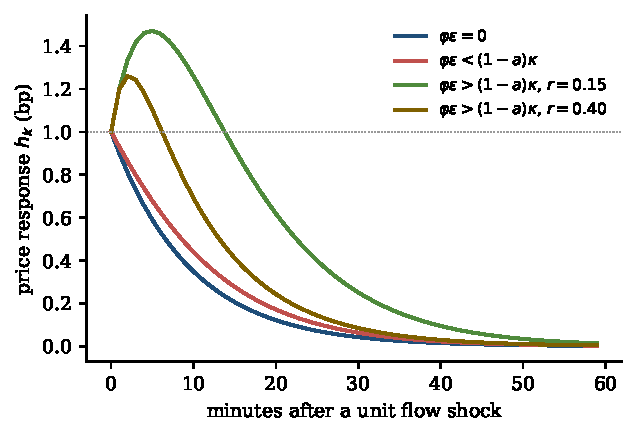
\includegraphics[width=0.6\textwidth]{figs/fig_t6.pdf}
\caption{Illustrative impulse responses of model \eqref{eq:x}--\eqref{eq:d} ($a=0.9$, $\kappa=1$, $\varepsilon=0.1$). The response overshoots only when $\varphi\varepsilon>(1-a)\kappa$; faster refill $r$ lowers the overshoot. Parameters are illustrative, not estimates.}\label{fig:t6}
\end{figure}

\subsection{Momentum traders}

Add momentum traders whose flow $f_t=(1-\eta)f_{t-1}+\eta q\,x_{t-1}$ enters both \eqref{eq:x} and \eqref{eq:d} alongside $u_t$.

\begin{proposition}[One-period amplification margin]\label{prop:t6m}
Let $C_3\equiv\varphi\varepsilon+\kappa^2\eta q-(1-a)\kappa$. Then $h_1-h_0=C_3$, so $C_3>0$ implies that the book amplifies.
\end{proposition}

\begin{proof}
With a unit shock at $t=0$, $x_0=\kappa$, $d_0=\varepsilon$ and $f_1=\eta q\kappa$, so $h_1=a\kappa+\varphi\varepsilon+\kappa^2\eta q$.
\end{proof}

With two slow modes the converse fails, and no condition on the one-period margin is exact. Three results describe what can be said instead.

\begin{theorem}[Momentum alone cannot make a stable book amplify]\label{thm:nomom}
Suppose $\varphi\varepsilon=0$ and $q\ge0$, and the system is stable. Then $h_k\le\kappa\,\rho^k<\kappa$ for every $k\ge1$, where $\rho<1$ is the spectral radius. In particular $C_3<0$.
\end{theorem}

\begin{proof}
Without the depth channel the state $(x_t,f_t)$ evolves by $M=\begin{psmallmatrix}a+\kappa\eta q&\kappa(1-\eta)\\ \eta q&1-\eta\end{psmallmatrix}$, which is entrywise nonnegative, and $h_k=\kappa(M^k)_{11}$. The off-diagonal product is nonnegative, so the eigenvalues are real, and by the Perron--Frobenius theorem $\lambda_2\le m_{11}\le\lambda_1=\rho$. Writing $(M^k)_{11}=c_1\lambda_1^k+c_2\lambda_2^k$ with $c_1=(m_{11}-\lambda_2)/(\lambda_1-\lambda_2)\in[0,1]$ and $c_2=1-c_1$ gives $(M^k)_{11}\le\rho^k$. Since $m_{11}\le\rho<1$, $C_3=\kappa(m_{11}-1)<0$.
\end{proof}

\begin{theorem}[A sufficient condition for no overshoot]\label{thm:noover}
For any signs of $\varphi$, $\varepsilon$ and $q$, if
\[
\bar C_3\equiv|\varphi\varepsilon|\Bigl(1+\frac{\kappa|q|}{r}\Bigr)+\kappa^2|q|-(1-a)\kappa\;\le\;0,
\]
then $\sup_k|h_k|=\kappa$: the response never exceeds its impact in either direction. When $\varphi\varepsilon\ge0$ and $q\ge0$, $C_3>0\Rightarrow$ amplification $\Rightarrow\bar C_3>0$.
\end{theorem}

\begin{proof}
Suppose $|x_j|\le\kappa$ for $j<k$. Then $|f_j|\le|q|\kappa$ for $j\le k$ and $|d_{k-1}|\le|\varepsilon|\bigl(b^{k-1}+\sum_{j\ge1}b^{k-1-j}|q|\kappa\bigr)\le|\varepsilon|(1+|q|\kappa/r)$, so $|x_k|\le a\kappa+|\varphi\varepsilon|(1+\kappa|q|/r)+\kappa^2|q|\le\kappa$. Induction from $x_0=\kappa$ completes the proof.
\end{proof}

\begin{remark}[Counterexamples to an exact one-period condition]\label{rem:counter}
Between $C_3$ and $\bar C_3$ the sign of $C_3$ does not decide. With $\kappa=1$, $a=0.98526$, $\varphi=0.7409$, $\varepsilon=0.01183$, $r=0.03436$, $\eta=0.5092$ and $q=0.01127$ (all channels reinforcing, $\rho=0.9995$), $C_3=-0.00024$ but the response peaks at lag 60 at $1.092\kappa$. With replenishment ($\varphi=2.614$, $\varepsilon=-0.405$, $a=0.9426$, $r=0.033$, $\eta=0.0016$, $q=0.0785$, $\rho=0.998$), $C_3=-1.11$ yet the response oscillates to $9.2\kappa$ at lag 90. In a search over 400{,}000 parameter draws such cases occur only near the stability boundary or with slow refill and slow momentum.
\end{remark}

\begin{proposition}[Summed response in closed form]\label{prop:sum}
Let $\tilde\kappa=\kappa+\varphi\varepsilon/r$ (long-run impact: direct plus depth) and $m=1-a$ (reversion). In the stable three-state model,
\[
S\equiv\sum_{k\ge0}h_k=\frac{\tilde\kappa}{m-q\tilde\kappa},
\]
and when $\varphi\varepsilon\ge0$ and $q\ge0$ the system is stable only if $m>q\tilde\kappa$. When all $h_k\ge0$, $S$ is the summed absolute response that enters the guard of Section~\ref{sec:guard}.
\end{proposition}

\begin{proof}
$S=e_1^\top(I-M_3)^{-1}(\kappa,\varepsilon,0)^\top$ with $M_3$ the transition matrix of $(x,d,f)$. Direct computation gives $\det(I-M_3)=\eta\,[\,r(m-\kappa q)-\varphi\varepsilon q\,]$ and the stated ratio; the formula matches the simulated sums to a relative error of $7\times10^{-14}$ in 3{,}000 stable draws.
\end{proof}

Cumulative transient risk is long-run impact divided by reversion net of momentum. Two practical consequences follow. First, the statistic that matters for losses is the summed response, which grows without bound as reversion falls to $q\tilde\kappa$, even when no single lag overshoots (Theorem~\ref{thm:nomom}). Second, $C_3$ is best read as a one-period amplification margin: it moves with $m$, $q$ and $\tilde\kappa$ in the same direction as $S$ and is what we estimate in Sections~\ref{sec:depth} and~\ref{sec:thin}. Both statistics are invariant in sign to rescaling flow.

\section{An identification-free pre-trade guard}\label{sec:guard}

\subsection{The quantity gate}
Observable dynamics are $z_{j+1}=Jz_j+Hv_j$ with loss output $l_t=Cz_t$ and executed quantities $|v_j|\le V$. Let $b_t=CJ^tz_0$ be the drift from past flow and $g^*_t=\max_{m<t}|c^\top_{\rm price}J^mH|$ the peak impulse gain up to $t$. Superposition gives, under a reserve $L_{\rm other}$ and execution cost $c_{\rm exec}$, the sharp allowance
\begin{equation}\label{eq:gate}
V^*=\min_{t:\,g^*_t+c_{\rm exec}>0}\frac{B-L_{\rm other}-|b_t|}{g^*_t+c_{\rm exec}},\qquad\bar R=V^*/\tau
\end{equation}
over a window of $\tau$ seconds. The gate needs only impulse coefficients and the current drift.

\subsection{Maximality}
A dealer with inventory $I$ chooses an admission level $\alpha\in[0,1]$ (the fraction of incoming algorithmic flow it accepts, or the depth it quotes). The closed-loop operator is $J(\alpha)=J_0+\alpha B_F$ with price impulse response $g_k(\alpha)$. Shocks satisfy $|u_t|\le\bar u$. Over horizon $H$ the price change is $\sum_{k<H}g_k(\alpha)u_{t-k}$, and the dealer has a loss budget $\mathcal B$.

\begin{theorem}[Summed-gain guard is maximal]\label{thm:guard}
The worst-case loss over horizon $H$ is
\[
L_{\max}(\alpha)=|I(\alpha)|\,\bar u\sum_{k<H}|g_k(\alpha)|.
\]
Hence the guard ``admit $\alpha$ iff $L_{\max}(\alpha)\le\mathcal B$'' is necessary and sufficient for bounded-shock solvency: it admits every safe $\alpha$ and no unsafe one. Replacing $\sum_k|g_k|$ by $\max_k|g_k|$ can admit unsafe levels; replacing it by $H\max_k|g_k|$ is safe but conservative.
\end{theorem}

\begin{proof}
By H\"older's inequality $|\sum_kg_ku_{t-k}|\le\bar u\sum_k|g_k|$, with equality for $u_{t-k}=\bar u\,{\rm sign}(g_k)$, which is admissible. Multiplying by $|I(\alpha)|$ gives $L_{\max}$, so the admission set equals the safe set. Since $\max_k|g_k|\le\sum_k|g_k|\le H\max_k|g_k|$, the peak guard under-states loss and the $H$-scaled guard over-states it.
\end{proof}

The worst-case identity in Theorem~\ref{thm:guard} is not new as mathematics: the induced $\ell_\infty$ gain of a linear convolution operator is the $\ell_1$ norm of its kernel, the fact on which $\ell_1$-optimal control of persistent bounded disturbances is built \citep{vidyasagar1986,dahleh1987,dahleh1995}. We use it rather than claim it. The finance content lies elsewhere: the dealer's admission level changes the operator itself, so the guard is a rule over an action set rather than a controller design; the bound is carried through margin, hedging and fill accounting (Theorem~\ref{thm:forward}); its single input is invariant to how the unobserved traders are split into cohorts and is identified from prices (Propositions~\ref{prop:invariance} and~\ref{prop:bridge}); the peak-response and eigenvalue rules it is compared with are the ones closest to current supervisory practice; and the same statistic prices the corrective rebate in equilibrium (Proposition~\ref{prop:equil}).

Numerically, the guard coincides with a brute-force adversary's maximal safe $\alpha$ in 200 of 200 random states. The peak-gain guard admitted an unsafe level in 2,000 of 2,000 states, the $H$-scaled guard was conservative in all 2,000, and $L_{\max}$ was non-decreasing in $\alpha$ in all 2,000, so the admission set was an interval in these examples.

\subsection{Computability: a finite-horizon certificate}

\begin{lemma}[Contraction-block tail bound]\label{lem:tail}
Let $\rho(J(\alpha))<1$. Suppose that at horizon $H$ there is a block length $H_0\le H$ with $q(\alpha)\equiv\|J(\alpha)^{H_0}\|_2<1$, and let $\bar M_{H_0}(\alpha)=\max_{0\le r<H_0}\|c^\top_{\rm price}J(\alpha)^r\|_2$ and $M_{C,H}(\alpha)=\max_{k\le H}\|c^\top_{\rm price}J(\alpha)^k\|_2$. Then
\begin{align}
\sup_{k\ge0}\|c^\top_{\rm price}J(\alpha)^k\|_2&\le\max\Bigl(M_{C,H}(\alpha),\ \bar M_{H_0}(\alpha)q(\alpha)^{\lfloor(H+1)/H_0\rfloor}\Bigr),\label{eq:tail}\\
G_{{\rm cum},\infty}(\alpha)&\le G_{{\rm cum},H}(\alpha)+\frac{\bar M_{H_0}(\alpha)H_0\,q(\alpha)^{\lfloor(H+1)/H_0\rfloor}}{1-q(\alpha)}.\notag
\end{align}
\end{lemma}

\begin{proof}
Write any $k>H$ as $k=mH_0+r$ with $m\ge\lfloor(H+1)/H_0\rfloor$ and $0\le r<H_0$. Submultiplicativity gives $\|c^\top J^k\|\le\|c^\top J^r\|\,\|J^{H_0}\|^m\le\bar M_{H_0}q^m$. Taking the supremum and summing the geometric tail gives \eqref{eq:tail}.
\end{proof}

The certificate turns an infinite-horizon supremum into a finite computation with a verified remainder. If the second term in the maximum is below $M_{C,H}$, truncation at $H$ is exact.

\subsection{Robustness to estimation error}

\begin{theorem}[Robust gain]\label{thm:robust}
Let $M=\sup_k\|J^k\|$ and $S=\sum_k\|J^k\|$. If $\|E\|\le\epsilon$ and $\epsilon S<1$, then $\sup_k\|(J+E)^k\|\le M/(1-\epsilon S)$.
\end{theorem}

\begin{proof}
Let $P_k=(J+E)^k$. Expanding, $P_k=J^k+\sum_{j<k}J^{k-1-j}EP_j$. With $m_k=\|P_k\|$, $m_k\le M+\epsilon\sum_{j<k}\|J^{k-1-j}\|m_j\le M+\epsilon S\max_{j<k}m_j$. Since $m_0=1\le M$, induction gives $m_k\le M/(1-\epsilon S)$ for all $k$.
\end{proof}

The bound held in all 30,000 random perturbations of 100 non-normal operators, with median tightness $0.50$ (realized gain over bound; maximum $0.57$). In a simulated window estimator of the kind used in Section~\ref{sec:spot} (600 transitions), a residual-bootstrap 95\% ball for the operator covered the true $J$ in $94.7\%$ of 300 replications, with median radius $0.086$; but $\epsilon S<1$ held in only $8\%$ of windows. The certificate is valid but often unavailable at realistic sample sizes; longer windows or pooled estimates are needed to use it in practice.

\begin{proposition}[No identification needed; numerical]\label{prop:bridge}
In a two-cohort economy with rates $0.7\pm\Delta$, the relative error of the estimated summed gain is flat in $\Delta$ (log--log slope $-0.15$), while the error of the cohort weights grows as $\Delta^{-3.07}$.
\end{proposition}

The guard needs the summed gain, which is cheap to estimate and invariant to cohort splitting (Proposition~\ref{prop:invariance}); it does not need the algorithms' identities, which are expensive \citep{niroula2026}.

\subsection{A calibrated illustration}\label{sec:calib}

How much does the choice between peak and summed guards matter in a real book? We compute the three-state impulse response at the median estimates of Section~\ref{sec:depth} (all training days and high-volatility days) and at a hypothetical book in which flow depletes the side it hits ($\varepsilon=+0.02$, other parameters at their high-volatility medians), Figure~\ref{fig:calib} and Table~\ref{tab:calib}.

\begin{figure}[t]\centering
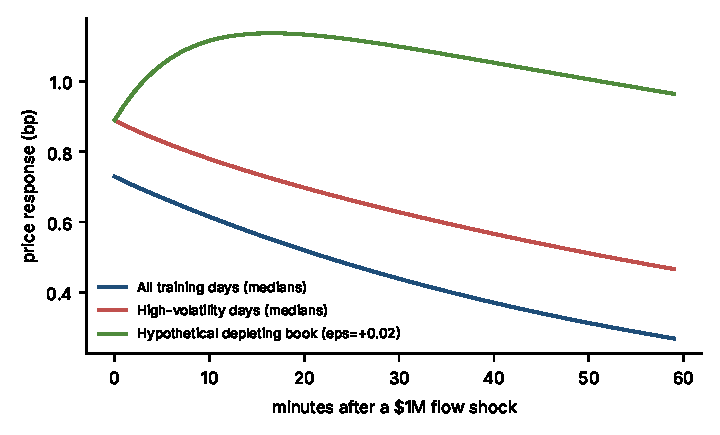
\includegraphics[width=0.62\textwidth]{figs/fig_calib.pdf}
\caption{Price response to a \$1M flow shock at the median depth estimates and in a hypothetical depleting book. Computed from the estimates of Table~\ref{tab:d3}.}\label{fig:calib}
\end{figure}

\begin{table}[t]\centering\small
\begin{threeparttable}
\caption{Peak versus summed gain at calibrated parameters}\label{tab:calib}
\setlength{\tabcolsep}{4pt}
\begin{tabular}{p{0.2\textwidth}ccccccc}
\toprule
Book & $C_3$ & Peak (min) & $\sum_{k<15}|g_k|$ & $\sum_{k<60}|g_k|$ & Sum/peak & Cap, peak & Cap, sum\\
\midrule
All days (medians) & $-0.013$ & 0.73 (0) & 9.73 & 27.67 & 13.3 & \$274M & \$21M\\
High-vol.\ days (medians) & $-0.014$ & 0.89 (0) & 12.17 & 38.71 & 13.7 & \$225M & \$16M\\
Depleting book ($\varepsilon=0.02$) & $+0.042$ & 1.14 (17) & 15.85 & 63.69 & 14.0 & \$176M & \$13M\\
\bottomrule
\end{tabular}
\begin{tablenotes}\footnotesize\item Gains in bp per \$1M of flow; sum/peak at 15 minutes. Inventory cap under a peak guard and under the summed guard, for a loss budget of \$100,000, an illustrative shock bound of \$5M of flow per minute and a 15-minute horizon. From \texttt{calib\_guard.py}, using the medians of Table~\ref{tab:d3}.\end{tablenotes}
\end{threeparttable}
\end{table}

The result is striking even though BTCUSDT does not amplify. Because price impact is persistent ($\hat a\approx0.97$ per minute), the summed gain over 15 minutes is about 13 times the peak. A guard calibrated to the peak would admit inventory about 13 times larger than is safe against a sustained adversarial flow of the declared size. Amplification makes this worse (the depleting book peaks 17 minutes after the shock), but persistence alone already makes peak-based limits unsafe. This is the practical content of Theorem~\ref{thm:guard} for this market.

\subsection{Two deployment modes}

\begin{enumerate}[label=\textbf{Mode \Alph*.},leftmargin=*]
\item \emph{An individual dealer.} A price-taking market maker with a small share of aggregate depth scales its own quote size by $\alpha$. This scales its passive fill intake but leaves aggregate depth, impact and the market operator unchanged.
\item \emph{A venue or sponsoring broker.} A gate at a matching engine or a market-access gateway (the setting of Rule 15c3-5) admits a fraction $\alpha$ of incoming aggressive algorithmic flow while resting depth stays posted. The operator becomes $J(\alpha)=A_0+\alpha B_F$.
\end{enumerate}

\paragraph{Algorithm (pre-trade guard).} At each step, using only pre-shock information:
\begin{enumerate}[itemsep=1pt]
\item For each $\alpha$ on a grid $\mathcal A=\{0,0.025,\ldots,1\}$, compute $\rho(J(\alpha))$, the peak and summed gains $M_{C,H}(\alpha)$ and $G_{{\rm cum},H}(\alpha)$, and the tail certificate of Lemma~\ref{lem:tail}; if an operator confidence radius $\epsilon$ is available, inflate by Theorem~\ref{thm:robust}.
\item Compute post-hedge and worst-case post-fill inventory, hedging cost and the post-fill margin increment.
\item Admit the largest $\alpha\in\mathcal A$ that satisfies the solvency inequalities of Theorem~\ref{thm:forward}; if none does, set $\alpha=0$, flag that no safe action exists, and trigger inventory reduction.
\end{enumerate}
For low-dimensional $J$ the grid evaluation is a sequence of matrix--vector products; execution takes well under one millisecond in compiled code, which we regard as an engineering detail rather than a result.

\subsection{Balance-sheet solvency}

\begin{theorem}[Conditional bounded-shock forward solvency]\label{thm:forward}
Consider a dealer with cash $K_t$, inventory $I_t$, mark $p_t$, equity $E_t=K_t+I_tp_t$, maintenance margin $MM_t=\max(0,\mu|I_t|p_t-c_0)$ and remaining buffer $B_{{\rm rem},t}=E_t-MM_t$, a safety reserve $R_{\rm safe}$, a hedge $\Delta I^{\rm hedge}_t(\alpha)$ with cost $C_{{\rm hedge},t}(\alpha)$, worst-case passive fills $\Delta I^{\rm fill}_{\max,t}(\alpha)$ with margin increment $C_{{\rm fill},t}(\alpha)$, and declared one-step and cumulative shock envelopes $\bar u_{{\rm step},t}\le\bar u_{{\rm cum},t}$. Let $|I^{\rm post}_{t+1}(\alpha)|=|I_t+\Delta I^{\rm hedge}_t(\alpha)|+\Delta I^{\rm fill}_{\max,t}(\alpha)$. Suppose the guard admits $\alpha_t$ only if
\begin{equation}\label{eq:guardineq}
|I^{\rm post}_{t+1}(\alpha_t)|(1+\mu)\Bigl(M_{C}(\alpha_t)\|z_t\|_2+s(\alpha_t)G_{\rm cum}(\alpha_t)\bar u_{{\rm cum},t}\Bigr)+C_{{\rm hedge},t}(\alpha_t)+C_{{\rm fill},t}(\alpha_t)+R_{\rm safe}\le B_{{\rm rem},t},
\end{equation}
where $s(\alpha)$ scales admitted shocks. Then for every disturbance path within the declared envelopes, the buffer after the step is at least $R_{\rm safe}$; by induction, solvency holds at every step at which an admissible $\alpha$ exists. At $\alpha=0$ the one-step admissible shock is
\[
\bar u_{{\rm adm},t}=\frac{B_{{\rm rem},t}-R_{\rm safe}-|I_t|(1+\mu)\|z_t\|_2}{|I_t|(1+\mu)} .
\]
The condition is sufficient over the whole disturbance ball. It is also necessary when the current state contributes no drift ($z_t=0$), because the shock term is then attained by adversarially signed disturbances; with $z_t\neq0$ the drift term $M_C\|z_t\|_2$ is an upper bound and the condition may be conservative. The admissible shock at $\alpha=0$ assumes, as in the cohort economy (Lemma~\ref{lem:cm}), that the price-row gain without admitted flow is $M_C(0)=1$.
\end{theorem}

Two features matter. The guard accounts for the inventory the dealer will hold after hedging and after worst-case fills, not only current inventory, and it never claims safety on an infeasible state: if no $\alpha$ satisfies \eqref{eq:guardineq}, it halts new fills and flags the state, because pre-existing inventory can still breach margin on a large adverse jump. In a constructed scenario ($E_0=10{,}000$, $I_0=-2{,}000$ at $P^*=100$, Tier-2 margin with $\mu=0.005$, buffer $9{,}050$ and reserve $950$), the admissible shock at $z_0=0$ is $8{,}100/2{,}010=4.03$ per unit, and an adversarial move of $4.05$ violates the reserve.

\begin{proposition}[When the guard beats an eigenvalue rule]\label{prop:dominance}
Let an eigenvalue guard admit $\alpha_\rho=\max\{\alpha:\rho(J(\alpha))\le\bar\rho\}$, and suppose the state is feasible for the summed-gain guard, which then admits at least $\alpha=0$. The eigenvalue guard admits a single-step breach that the summed-gain guard prevents if and only if
\[
M_C(\alpha_\rho)\;>\;\frac{B_{{\rm rem},t}-R_{\rm safe}-C_{{\rm hedge},t}(\alpha_\rho)-C_{{\rm fill},t}(\alpha_\rho)}{|I^{\rm post}_{t+1}(\alpha_\rho)|(1+\mu)(\|z_t\|_2+s(\alpha_\rho)\bar u_{{\rm step},t})} .
\]
\end{proposition}

The eigenvalue rule fails exactly when the transient gain at its admitted level exceeds the loss the balance sheet can absorb, which Proposition~\ref{prop:blind} shows can happen at any spectral threshold.

\begin{proposition}[Strategic re-optimization reinforces the guard]\label{prop:lucas}
Suppose cohorts re-optimize their steady-state Kalman gains when the venue throttles admission, and throttling scales the variance of execution-driven innovations as $\sigma_\zeta^2(\alpha)=\alpha^2\sigma_{\zeta,0}^2$ while measurement noise $\sigma_\nu^2>0$ is unchanged. Then the optimal gain $\eta^*(\alpha)$ is strictly increasing in $\alpha$, so throttling lowers every cohort's adaptation rate. If the transient gain is non-decreasing in the adaptation rates, then $M_C(J(\alpha,\eta^*(\alpha)))\le M_C(J(\alpha,\eta^*(1)))$: re-optimization does not undo the guard.
\end{proposition}

The first statement is a property of the Riccati root; the second is conditional on monotonicity of the gain in $\eta$, which we check numerically. Across 3{,}000 stable draws of the three-state book with momentum (adaptation rates on a grid from 0.05 to 0.95), the peak response is non-decreasing in $\eta$ in 98.8\% of draws and in 99.9\% of those with trend-following cohorts ($q>0$); the summed absolute response is non-decreasing in 93\% of draws with $q>0$ but decreasing when cohorts are contrarian ($q<0$). For trend-following cohorts, the case the filtering microfoundation produces, re-optimization therefore reinforces the guard in almost every case we drew; the signed sum $S$ of Proposition~\ref{prop:sum} does not depend on $\eta$ at all (\texttt{recompute\_oct20.py}). A manipulator who instead increases order size to offset throttling enlarges the shock envelope and drives $\alpha$ toward zero.
